%% LyX 2.3.7 created this file.  For more info, see http://www.lyx.org/.
%% Do not edit unless you really know what you are doing.
\documentclass[journal,article,submit,pdftex,moreauthors]{Definitions/mdpi}
\usepackage[utf8]{inputenc}
\usepackage{float}
\usepackage{url}
\usepackage{amsmath}
\usepackage{graphicx}

\makeatletter

%%%%%%%%%%%%%%%%%%%%%%%%%%%%%% LyX specific LaTeX commands.

\Title{EOFA: an extended version of the optimal foraging algorithm for global
optimization problems}

\TitleCitation{EOFA: an extended version of the optimal foraging algorithm for global
optimization problems}

\Author{Glykeria Kyrou$^{1}$, Vasileios Charilogis$^{2}$ and Ioannis G.
Tsoulos$^{3,*}$}

\AuthorNames{Glykeria Kyrou, Vasileios Charilogis and Ioannis G. Tsoulos }

\AuthorCitation{Kyrou, G.; Charilogis, V.; Tsoulos, I.G. }


\address{$^{1}$\quad{}Department of Informatics and Telecommunications,
University of Ioannina, 47150 Kostaki Artas, Greece; g.kyrou@uoi.gr\\
$^{2}$\quad{}Department of Informatics and Telecommunications, University
of Ioannina, 47150 Kostaki Artas, Greece; v.charilog@uoi.gr\\
$^{3}\quad$Department of Informatics and Telecommunications, University
of Ioannina, 47150 Kostaki Artas, Greece;itsoulos@uoi.gr}


\corres{Correspondence: itsoulos@uoi.gr}


\abstract{The problem of finding the global minimum of a function is applicable
to a multitude of real-world problems, and for this reason a variety
of computational techniques have been developed to efficiently locate
it. Among these techniques, evolutionary techniques play a central
role, which seek, through the imitation of natural processes, to efficiently
obtain the global minimum of multidimensional functions. An evolutionary
technique that has recently been introduced is the optimal foraging
algorithm, which is a swarm - based algorithm, and it is notable for
its reliability in locating the global minimum. In this work, a series
of modifications are proposed that aim to improve the reliability
and speed of the above technique, such as a termination technique
based on stochastic observations, an innovative sampling method and
a technique to improve the generation of offspring. The new method
was tested on a series of problems from the relevant literature and
a comparative study was made against other global optimization techniques
with promising results. }


\keyword{Global optimization; Stochastic techniques; Evolutionary methods;
Swarm based methods}

\DeclareTextSymbolDefault{\textquotedbl}{T1}
%% Because html converters don't know tabularnewline
\providecommand{\tabularnewline}{\\}

%%%%%%%%%%%%%%%%%%%%%%%%%%%%%% User specified LaTeX commands.
%  LaTeX support: latex@mdpi.com 
%  For support, please attach all files needed for compiling as well as the log file, and specify your operating system, LaTeX version, and LaTeX editor.

%=================================================================


% For posting an early version of this manuscript as a preprint, you may use "preprints" as the journal and change "submit" to "accept". The document class line would be, e.g., \documentclass[preprints,article,accept,moreauthors,pdftex]{mdpi}. This is especially recommended for submission to arXiv, where line numbers should be removed before posting. For preprints.org, the editorial staff will make this change immediately prior to posting.

%--------------------
% Class Options:
%--------------------
%----------
% journal
%----------
% Choose between the following MDPI journals:
% acoustics, actuators, addictions, admsci, adolescents, aerospace, agriculture, agriengineering, agronomy, ai, algorithms, allergies, alloys, analytica, animals, antibiotics, antibodies, antioxidants, applbiosci, appliedchem, appliedmath, applmech, applmicrobiol, applnano, applsci, aquacj, architecture, arts, asc, asi, astronomy, atmosphere, atoms, audiolres, automation, axioms, bacteria, batteries, bdcc, behavsci, beverages, biochem, bioengineering, biologics, biology, biomass, biomechanics, biomed, biomedicines, biomedinformatics, biomimetics, biomolecules, biophysica, biosensors, biotech, birds, bloods, blsf, brainsci, breath, buildings, businesses, cancers, carbon, cardiogenetics, catalysts, cells, ceramics, challenges, chemengineering, chemistry, chemosensors, chemproc, children, chips, cimb, civileng, cleantechnol, climate, clinpract, clockssleep, cmd, coasts, coatings, colloids, colorants, commodities, compounds, computation, computers, condensedmatter, conservation, constrmater, cosmetics, covid, crops, cryptography, crystals, csmf, ctn, curroncol, currophthalmol, cyber, dairy, data, dentistry, dermato, dermatopathology, designs, diabetology, diagnostics, dietetics, digital, disabilities, diseases, diversity, dna, drones, dynamics, earth, ebj, ecologies, econometrics, economies, education, ejihpe, electricity, electrochem, electronicmat, electronics, encyclopedia, endocrines, energies, eng, engproc, ent, entomology, entropy, environments, environsciproc, epidemiologia, epigenomes, est, fermentation, fibers, fintech, fire, fishes, fluids, foods, forecasting, forensicsci, forests, foundations, fractalfract, fuels, futureinternet, futureparasites, futurepharmacol, futurephys, futuretransp, galaxies, games, gases, gastroent, gastrointestdisord, gels, genealogy, genes, geographies, geohazards, geomatics, geosciences, geotechnics, geriatrics, hazardousmatters, healthcare, hearts, hemato, heritage, highthroughput, histories, horticulturae, humanities, humans, hydrobiology, hydrogen, hydrology, hygiene, idr, ijerph, ijfs, ijgi, ijms, ijns, ijtm, ijtpp, immuno, informatics, information, infrastructures, inorganics, insects, instruments, inventions, iot, j, jal, jcdd, jcm, jcp, jcs, jdb, jeta, jfb, jfmk, jimaging, jintelligence, jlpea, jmmp, jmp, jmse, jne, jnt, jof, joitmc, jor, journalmedia, jox, jpm, jrfm, jsan, jtaer, jzbg, kidney, kidneydial, knowledge, land, languages, laws, life, liquids, literature, livers, logics, logistics, lubricants, lymphatics, machines, macromol, magnetism, magnetochemistry, make, marinedrugs, materials, materproc, mathematics, mca, measurements, medicina, medicines, medsci, membranes, merits, metabolites, metals, meteorology, methane, metrology, micro, microarrays, microbiolres, micromachines, microorganisms, microplastics, minerals, mining, modelling, molbank, molecules, mps, msf, mti, muscles, nanoenergyadv, nanomanufacturing, nanomaterials, ncrna, network, neuroglia, neurolint, neurosci, nitrogen, notspecified, nri, nursrep, nutraceuticals, nutrients, obesities, oceans, ohbm, onco, oncopathology, optics, oral, organics, organoids, osteology, oxygen, parasites, parasitologia, particles, pathogens, pathophysiology, pediatrrep, pharmaceuticals, pharmaceutics, pharmacoepidemiology, pharmacy, philosophies, photochem, photonics, phycology, physchem, physics, physiologia, plants, plasma, pollutants, polymers, polysaccharides, poultry, powders, preprints, proceedings, processes, prosthesis, proteomes, psf, psych, psychiatryint, psychoactives, publications, quantumrep, quaternary, qubs, radiation, reactions, recycling, regeneration, religions, remotesensing, reports, reprodmed, resources, rheumato, risks, robotics, ruminants, safety, sci, scipharm, seeds, sensors, separations, sexes, signals, sinusitis, skins, smartcities, sna, societies, socsci, software, soilsystems, solar, solids, sports, standards, stats, stresses, surfaces, surgeries, suschem, sustainability, symmetry, synbio, systems, taxonomy, technologies, telecom, test, textiles, thalassrep, thermo, tomography, tourismhosp, toxics, toxins, transplantology, transportation, traumacare, traumas, tropicalmed, universe, urbansci, uro, vaccines, vehicles, venereology, vetsci, vibration, viruses, vision, waste, water, wem, wevj, wind, women, world, youth, zoonoticdis 

%---------
% article
%---------
% The default type of manuscript is "article", but can be replaced by: 
% abstract, addendum, article, book, bookreview, briefreport, casereport, comment, commentary, communication, conferenceproceedings, correction, conferencereport, entry, expressionofconcern, extendedabstract, datadescriptor, editorial, essay, erratum, hypothesis, interestingimage, obituary, opinion, projectreport, reply, retraction, review, perspective, protocol, shortnote, studyprotocol, systematicreview, supfile, technicalnote, viewpoint, guidelines, registeredreport, tutorial
% supfile = supplementary materials

%----------
% submit
%----------
% The class option "submit" will be changed to "accept" by the Editorial Office when the paper is accepted. This will only make changes to the frontpage (e.g., the logo of the journal will get visible), the headings, and the copyright information. Also, line numbering will be removed. Journal info and pagination for accepted papers will also be assigned by the Editorial Office.

%------------------
% moreauthors
%------------------
% If there is only one author the class option oneauthor should be used. Otherwise use the class option moreauthors.

%---------
% pdftex
%---------
% The option pdftex is for use with pdfLaTeX. If eps figures are used, remove the option pdftex and use LaTeX and dvi2pdf.

%=================================================================
% MDPI internal commands - do not modify
\firstpage{1} 
 
\setcounter{page}{\@firstpage} 

\pubvolume{1}
\issuenum{1}
\articlenumber{0}
\pubyear{2024}
\copyrightyear{2024}
%\externaleditor{Academic Editor: Firstname Lastname} % For journal Automation, please change Academic Editor to "Communicated by"
\datereceived{}
\daterevised{ } % Comment out if no revised date
\dateaccepted{}
\datepublished{}
%\datecorrected{} % Corrected papers include a "Corrected: XXX" date in the original paper.
%\dateretracted{} % Corrected papers include a "Retracted: XXX" date in the original paper.
\hreflink{https://doi.org/} % If needed use \linebreak
%\doinum{}
%------------------------------------------------------------------
% The following line should be uncommented if the LaTeX file is uploaded to arXiv.org
%\pdfoutput=1

%=================================================================
% Add packages and commands here. The following packages are loaded in our class file: fontenc, inputenc, calc, indentfirst, fancyhdr, graphicx, epstopdf, lastpage, ifthen, lineno, float, amsmath, setspace, enumitem, mathpazo, booktabs, titlesec, etoolbox, tabto, xcolor, soul, multirow, microtype, tikz, totcount, changepage, attrib, upgreek, cleveref, amsthm, hyphenat, natbib, hyperref, footmisc, url, geometry, newfloat, caption

%=================================================================
%% Please use the following mathematics environments: Theorem, Lemma, Corollary, Proposition, Characterization, Property, Problem, Example, ExamplesandDefinitions, Hypothesis, Remark, Definition, Notation, Assumption
%% For proofs, please use the proof environment (the amsthm package is loaded by the MDPI class).

%=================================================================
% The fields PACS, MSC, and JEL may be left empty or commented out if not applicable
%\PACS{J0101}
%\MSC{}
%\JEL{}

%%%%%%%%%%%%%%%%%%%%%%%%%%%%%%%%%%%%%%%%%%
% Only for the journal Diversity
%\LSID{\url{http://}}

%%%%%%%%%%%%%%%%%%%%%%%%%%%%%%%%%%%%%%%%%%
% Only for the journal Applied Sciences:
%\featuredapplication{Authors are encouraged to provide a concise description of the specific application or a potential application of the work. This section is not mandatory.}
%%%%%%%%%%%%%%%%%%%%%%%%%%%%%%%%%%%%%%%%%%

%%%%%%%%%%%%%%%%%%%%%%%%%%%%%%%%%%%%%%%%%%
% Only for the journal Data:
%\dataset{DOI number or link to the deposited data set in cases where the data set is published or set to be published separately. If the data set is submitted and will be published as a supplement to this paper in the journal Data, this field will be filled by the editors of the journal. In this case, please make sure to submit the data set as a supplement when entering your manuscript into our manuscript editorial system.}

%\datasetlicense{license under which the data set is made available (CC0, CC-BY, CC-BY-SA, CC-BY-NC, etc.)}

%%%%%%%%%%%%%%%%%%%%%%%%%%%%%%%%%%%%%%%%%%
% Only for the journal Toxins
%\keycontribution{The breakthroughs or highlights of the manuscript. Authors can write one or two sentences to describe the most important part of the paper.}

%%%%%%%%%%%%%%%%%%%%%%%%%%%%%%%%%%%%%%%%%%
% Only for the journal Encyclopedia
%\encyclopediadef{Instead of the abstract}
%\entrylink{The Link to this entry published on the encyclopedia platform.}
%%%%%%%%%%%%%%%%%%%%%%%%%%%%%%%%%%%%%%%%%%

%%%%%%%%%%%%%%%%%%%%%%%%%%%%%%%%%%%%%%%%%%
% Only for the journal Advances in Respiratory Medicine
%\addhighlights{yes}
%\renewcommand{\addhighlights}{%

%\noindent This is an obligatory section in “Advances in Respiratory Medicine”, whose goal is to increase the discoverability and readability of the article via search engines and other scholars. Highlights should not be a copy of the abstract, but a simple text allowing the reader to quickly and simplified find out what the article is about and what can be cited from it. Each of these parts should be devoted up to 2~bullet points.\vspace{3pt}\\
%\textbf{What are the main findings?}
% \begin{itemize}[labelsep=2.5mm,topsep=-3pt]
% \item First bullet.
% \item Second bullet.
% \end{itemize}\vspace{3pt}
%\textbf{What is the implication of the main finding?}
% \begin{itemize}[labelsep=2.5mm,topsep=-3pt]
% \item First bullet.
% \item Second bullet.
% \end{itemize}
%}
%%%%%%%%%%%%%%%%%%%%%%%%%%%%%%%%%%%%%%%%%%

\makeatother

\begin{document}
\maketitle

\section{Introduction}

The basic goal of global optimization is to find the global minimum
by searching for the appropriate scope of each problem. Primarily,
a global optimization method aims to discover the global minimum of
a continuous function, and it is defined as

\begin{equation}
x^{*}=\mbox{arg}\min_{x\in S}f(x)\label{eq:eq1}
\end{equation}
with $S$: 
\[
S=\left[a_{1},b_{1}\right]\times\left[a_{2},b_{2}\right]\times\ldots\left[a_{n},b_{n}\right]
\]
Global optimization is a core part of applied mathematics \citep{math}
and computer science \citep{torn_stochastic}. Additionally, it finds
application in various fields such as physics \citep{go_physics1,go_physics2,go_physics3},
chemistry \citep{go_chem1,go_chem2,go_chem3}, economics \citep{go_econ1,go_econ2},
medicine \citep{go_med1,go_med2} etc. Optimization methods are divided
into deterministic and stochastic \citep{go_comparison}. Deterministic
methods guarantee finding the global optimal solution and are usually
applied to small problems \citep{go_det_vs_stochastic}. The most
commonly appeared techniques of the first category are the so - called
interval techniques \citep{interval1,interval2}, which divide the
initial domain of the function until it discovers a promising subset
that may contain the global minimum. On the other hand, stochastic
methods do not guarantee finding the global optimization and are mainly
applied to large problems, but are inefficient when nonlinear equality
constraints are involved. Stochastic methods include a variety of
techniques, such as Controlled Random Search methods \citep{crs1,crs2,crs3},
Simulated Annealing methods \citep{simann_major,simann1,simann2},
methods based on the Multistart technique \citep{mult_repulsion,mult_minfinder,mult_cfo}
etc. Also, in the recent literature, a variety of hybrid methods have
appeared that combine different optimization techniques \citep{mshybrid1,mshybrid2}.
Furthermore, due to the widespread usage of parallel programming architectures,
a variety of methods have been proposed that take advantage of such
systems \citep{parallel-multistart,parallel-multistart2,msgpu1,msgpu2}. 

An important group of stochastic techniques that has attracted the
interest of many researchers is the group of evolutionary techniques.
The branch of evolutionary computing includes the study of foundations
and applications of computational techniques based on the principles
of natural evolution. Evolution in nature is responsible for the \textquotedbl design\textquotedbl{}
of all living things on earth and the strategies they use to interact
with each other. This branch of methods includes Differential Evolution
methods \citep{diffe1,diffe2}, Particle Swarm Optimization (PSO)
methods \citep{pso_major,pso1,pso2}, Ant Colony optimization methods
\citep{aco1,aco2}, Genetic algorithms \citep{genetic1,genetic2}
etc. Zhu and Zhang proposed a novel method in this area, that tackles
optimization problems with a strategy based on the animal foraging
behavior \citep{ofa}. This Optimal Foraging Algorithm (OFA)\textbf{
}is a swarm-based algorithm motivated by animal behavioral ecology.
Also, Fu et al. proposed a variation of the OFA algorithm with the
incorporation of the Differential Evolution technique \citep{ofa_de}.
Additionally, Jian and Zhu proposed a modification of the OFA algorithm
with direction prediction \citep{ofa_pred} in order to enhance the
performance of the original algorithm.\textbf{ }Recently, Chen Ding
and Guang Yu Zhu introduced an improved quasi-adversarial optimal
social behavior search algorithm (QOS-OFA) to handle optimization
problems \citep{ofa_improved}.

The current work introduces a series of modifications to the OFA algorithm
in order to speed up the process and to increase the effectiveness
of the algorithm. These modifications include:
\begin{itemize}
\item Incorporation of a sampling technique that utilizes the K-Means method
\citep{kmeansNew}. The points that will be sampled will more accurately
and quickly lead to the global minimum of the function and additional
points that might have been close enough using another sampling technique
will be discarded. 
\item Use a termination technique based on stochastic observations. At each
iteration of the algorithm, the smallest functional value is recorded.
If this remains constant for a predetermined number of iterations,
then the method terminates. This way, the method will terminate in
time without needlessly wasting computing time on iterations that
will simply produce the same result. 
\item Improving the offspring produced by the method using a few steps of
a local minimization method. In the current work, a BFGS variant \citep{Powell}
was used as a local search procedure.
\end{itemize}
The rest of this paper is divided into the following sections: in
section \ref{sec:Materials-and-Methods} the proposed method is fully
described, in section \ref{sec:Results} the benchmark functions are
presented as well as the experimental results and finally in section
\ref{sec:Conclusions} some conclusions and guidelines for future
work are discussed.

\section{The proposed method\label{sec:Materials-and-Methods}}

The OFA algorithm uses nature as a source of inspiration. The OFA
algorithm has as its main purpose the evolution of the population
using some iterative steps which will be presented in more detail
below. The quality of the initial population can be improved, allowing
the search space to be explored more efficiently. The first major
modification introduced to the above technique is the use of a sophisticated
technique of sampling points from the objective function. This sampling
is based on the K-means technique and is presented in detail in the
subsection \ref{subsec:The-proposed-sampling}. The second modification
is to apply a few steps of a local search procedure in offspring creation,
if an offspring is not consistent with the bounds $[a,b]$ of the
objective function $f(x)$. With this modification, it is ensured
that a new point will be within the field definition of the function
on the one hand, and on the other hand, it will have a slightly lower
value than its predecessor. The third modification is to use an efficient
termination rule to terminate the global optimization method effectively.
This termination rule is outlined in subsection \ref{subsec:The-used-termination}.

\subsection{The main steps of the algorithm}

The main steps of the used global optimization method are the following:
\begin{enumerate}
\item \textbf{Initialization step}.
\begin{enumerate}
\item \textbf{Define} as $N_{c}$ the number of elements in the population.
\item \textbf{Define} as $N_{g}$ the maximum number of allowed iterations.
\item \textbf{Initialize} randomly the members of the population in set
$S$. This forms the initial population denoted as $P$. The sampling
is performed using the procedure of subsection \ref{subsec:The-proposed-sampling}.
\item \textbf{Create} the QOP population, that stands for the quasi-opposite
population of $P$, by calculating the quasi-opposite positions of
P .
\item \textbf{Set} $t=0$, the iteration number.
\item \textbf{Select} the $N_{c}$ fittest solutions from the population
set $\left\{ P,\text{\mbox{QOP}}\right\} $ using the QOBL method
proposed in \citep{ofa_improved}.
\end{enumerate}
\item \textbf{Calculation step}.
\begin{enumerate}
\item \textbf{Produce} the new offspring solutions $x^{t+1}$ based on the
ranking order using the following equation:
\begin{equation}
x_{j}^{t+1}=\begin{cases}
\begin{array}{cc}
x_{j}^{t}+K(t)\times\left(r_{1}-r_{2}\right)\times\left(x_{j}^{t}-x_{b}^{t}\right)+\left(1-K(t)\right)\times\left(x_{1}^{t}-x_{r}^{t}\right) & ,\ j=2,\ldots,N_{c}\\
x_{1}^{t}+K(t)\times\left(r_{1}-r_{2}\right)\times\left(x_{1}^{t}-x_{N_{c}}^{t}\right) & ,\ j=1
\end{array}\end{cases}
\end{equation}
where $r_{1},r_{2}$ are random numbers in $[0,1]$ and $x_{r}^{t}$
is a randomly selected solution from the population. The function
$K(t)$ is defined as
\begin{equation}
K(t)=\cos\left(\frac{\pi t}{2N_{g}}\right)
\end{equation}
\item \textbf{For} $j=1,\ldots,N_{c}$ \textbf{do}
\begin{enumerate}
\item \textbf{If} $x^{t+1}\ \notin S$ then $x^{t+1}=\mbox{LS}\left(x^{t},B_{i}\right)$.
This step applies a limited number of steps of a local search procedure
LS(x) to the current point. The parameter $B_{i}$ denotes the number
of steps for the local search procedure. In the current work the BFGS
local optimization procedure have been used, but other local search
methods could be employed such as Gradient Descent \citep{gd}, Steepest
Descent \citep{steepest} etc.
\item \textbf{if} $\ \frac{\lambda_{j}^{t+1}\times f\left(x^{t+1}\right)}{1+(t+1)\times\lambda_{j}^{t+1}}<\frac{f\left(x^{t}\right)}{t}$
then select $x^{t+1}$ for the next population else select $x^{t}$.
The values $\lambda_{j}^{t+1}$ are uniformly distributed random numbers
in $[0,1]$.
\end{enumerate}
\item \textbf{End For}
\item \textbf{Sort} all solutions in the current population fro the best
to worst according to the function value.
\end{enumerate}
\item \textbf{Termination check step}.
\begin{enumerate}
\item \textbf{Set} $t=t+1$
\item \textbf{Calculate} to stopping rule in the work of Charilogis \citep{stopping rule2}.
This termination method is described in subsection \ref{subsec:The-used-termination}.
\item \textbf{If} the termination criteria are not met then go to Calculation
step, \textbf{else} terminate.
\end{enumerate}
\end{enumerate}
The steps of the proposed method are also graphically shown in Figure
\ref{fig:ofaAlgorithm}.

\begin{figure}[H]
\begin{centering}
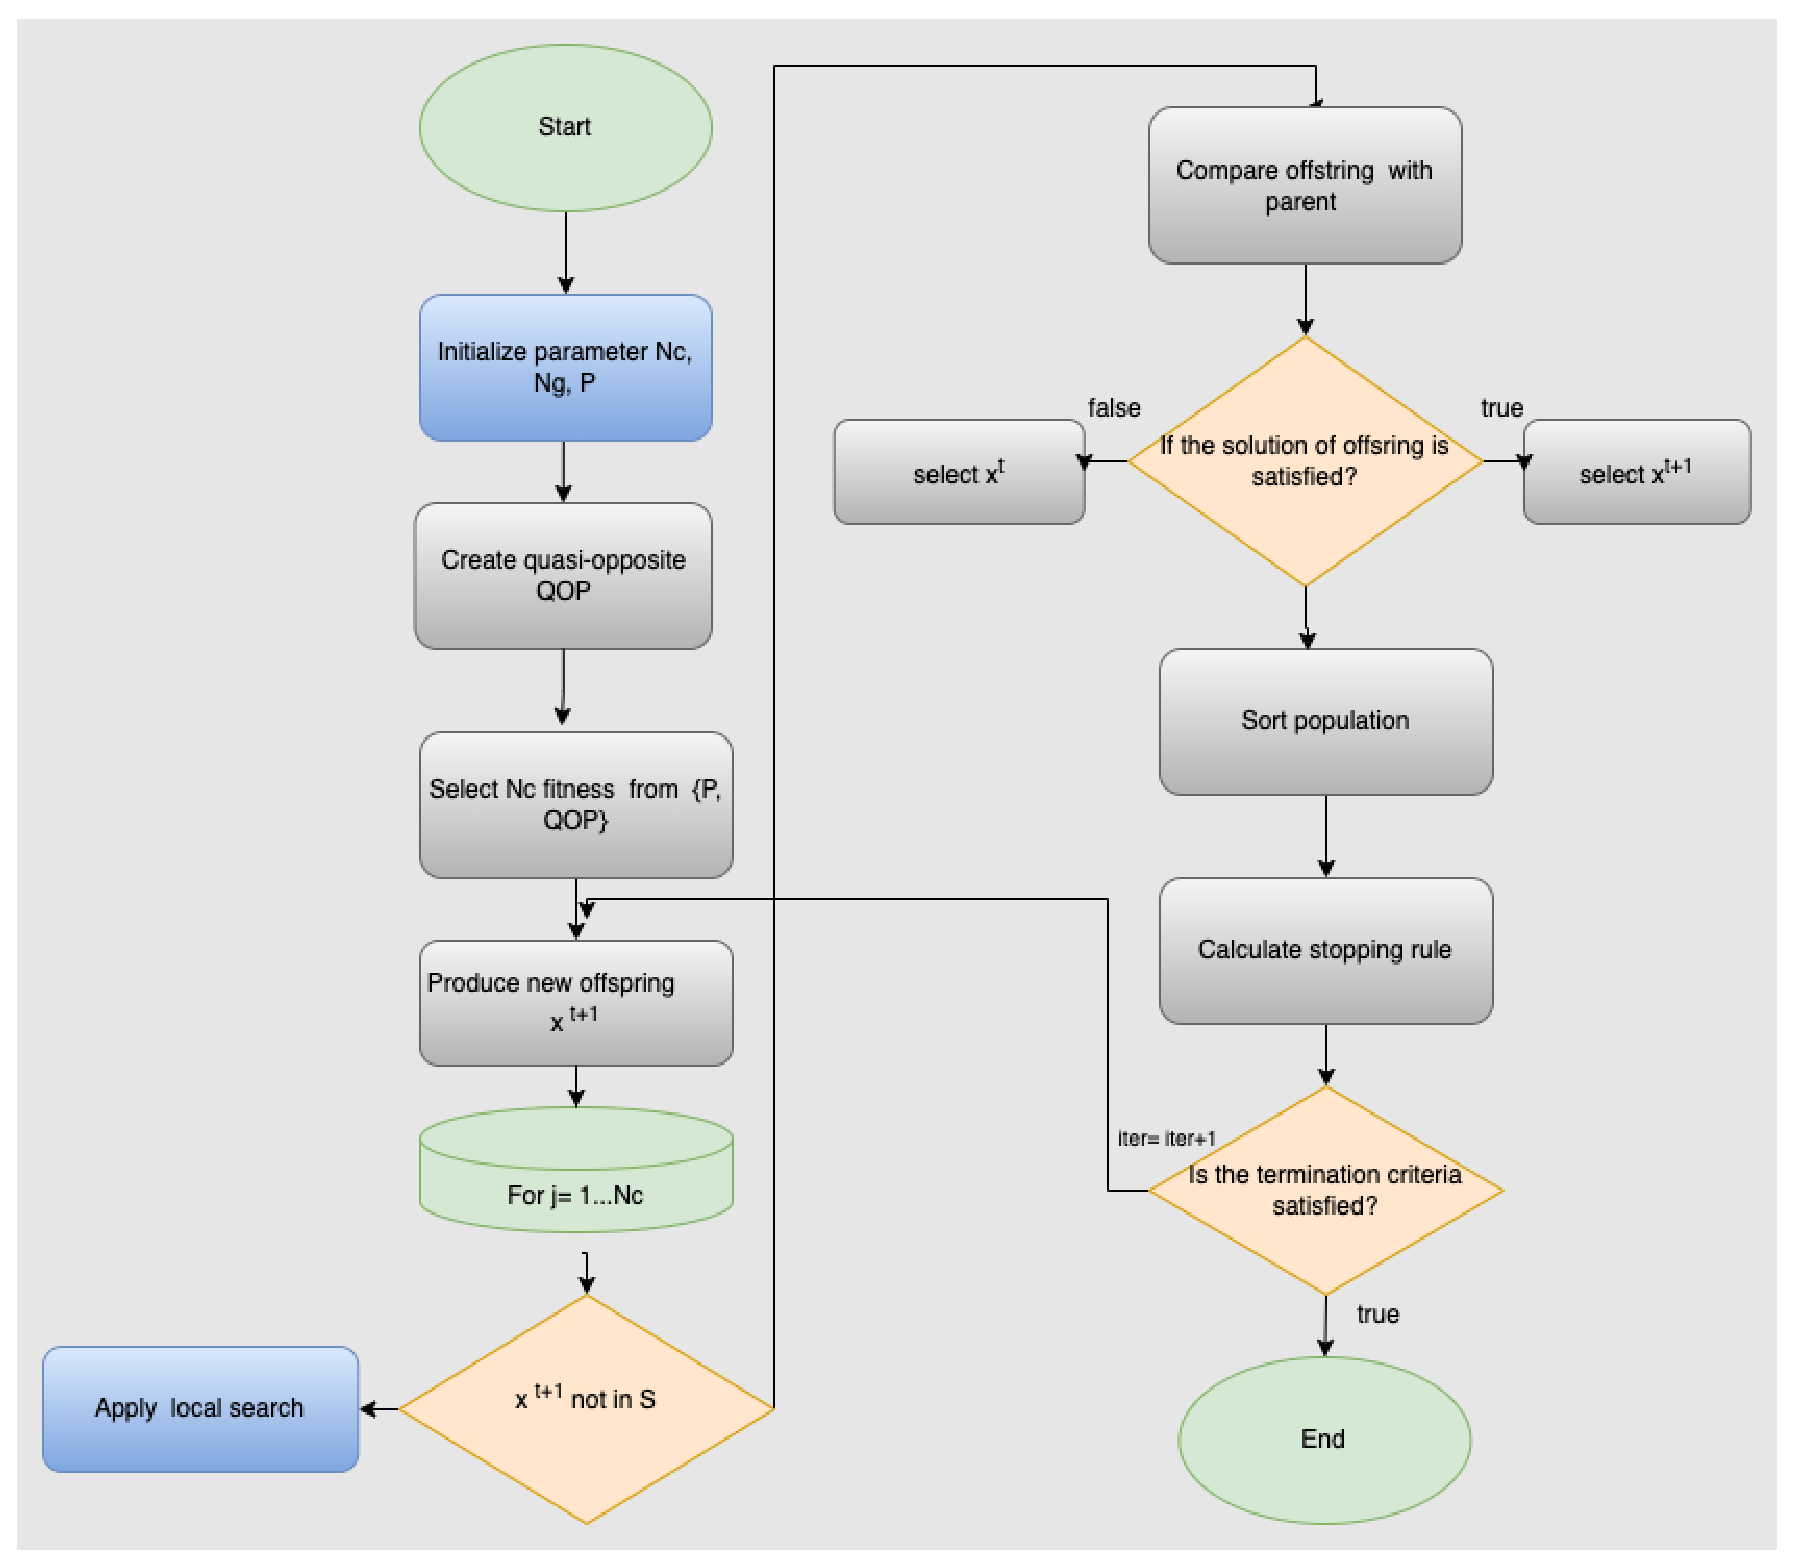
\includegraphics[scale=0.4]{ofa.eps}
\par\end{centering}
\caption{The steps of the proposed method as a series of steps.\label{fig:ofaAlgorithm}}

\end{figure}


\subsection{The proposed sampling procedure\label{subsec:The-proposed-sampling}}

The proposed sampling technique produces initially a series of samples
from the objective function and subsequently, through the application
of the K-means technique, only the located centers are considered
as the final samples. The method was introduced by James MacQueen\citep{MacQueen}
and it is a clustering algorithm that has been used in data analysis
and machine learning in a variety of research papers \citep{kmeans1,kmeans2}.\textbf{
}The algorithm seeks to estimate the centers of possible teams in
a set of samples and its main steps are listed subsequently:
\begin{enumerate}
\item \textbf{Define} as $k$ the number of clusters.
\item \textbf{Draw} randomly $N_{m}$ initial points $x_{i},\ i=1,\ldots,N_{m}$
from the objective function.
\item \textbf{Assign }randomly each point $x_{i},\ i=1,...,N_{m}$ in a
cluster $S_{j},\ j=1,\ldots,k$.
\item \textbf{For} every cluster $j=1..k$ \textbf{do}
\begin{enumerate}
\item \textbf{Set} as $M_{j}$ the number of points in $S_{j}$
\item \textbf{Compute }the center of the cluster $c_{j}$ as
\[
c_{j}=\frac{1}{M_{j}}\sum_{x_{i}\in S_{j}}x_{i}
\]
\end{enumerate}
\item \textbf{EndFor}
\item \textbf{Repeat}
\begin{enumerate}
\item Set $S_{j}=\left\{ \right\} ,\ j=1..k$
\item \textbf{For} each point $x_{i},\ i=1,...,N_{m}$ \textbf{do}
\begin{enumerate}
\item \textbf{Set} $j^{*}=\mbox{argmin}_{m=1}^{k}\left\{ D\left(x_{i},c_{m}\right)\right\} $.
The function $D(x,y)$ is the Euclidean distance of points $(x,y)$.
\item \textbf{Set} $S_{j^{*}}=S_{j^{*}}\cup\left\{ x_{i}\right\} $.
\end{enumerate}
\item \textbf{EndFor}
\item \textbf{For} each center $c_{j},\ j=1..k$ \textbf{do}
\begin{enumerate}
\item \textbf{Update }the center $c_{j}$ as
\[
c_{j}=\frac{1}{M_{j}}\sum_{x_{i}\in S_{j}}x_{i}
\]
\end{enumerate}
\item \textbf{EndFor}
\end{enumerate}
\item \textbf{If }there is no significant change in centers $c_{j}$\textbf{
terminate }the algorithm and return the $k$ centers as the final
set of samples.
\end{enumerate}

\subsection{The used termination rule\label{subsec:The-used-termination}}

At every iteration $t$, the difference between the current best value
$f_{min}^{(t)}$ and the previous best value $f_{min}^{(t-1)}$ is
computed:
\begin{center}
\begin{equation}
\delta^{(t)}=\left|f_{\mbox{min}}^{(k)}-f_{\mbox{min}}^{(k-1)}\right|\label{eq:best}
\end{equation}
\par\end{center}

The algorithm terminates when $\delta^{(t)}\le\epsilon$ for series
of predefined consecutive iterations $N_{k}$, where $\epsilon$ is
a small positive number, for example $10^{-6}$.

\section{Results\label{sec:Results}}

This section will begin with a detailed description of the functions
that will be used in the experiments, followed by an analysis of the
experiments performed and comparisons with other global optimization
techniques. 

\subsection{Test functions }

The functions used in the experiments have been proposed in a series
of relative works \citep{Ali1,Floudas1} and they cover various scientific
fields, such as medicine, physics, engineering, etc. Also, these objective
functions have been used by many researchers in a variety of publications
\citep{testfunctions1,testfunctions2,testfunctions3,testfunctions4}.
The definition of the test functions are given below:
\begin{itemize}
\item \textbf{Bf1} (Bohachevsky 1) function:
\end{itemize}
\[
f(x)=x_{1}^{2}+2x_{2}^{2}-\frac{3}{10}\cos\left(3\pi x_{1}\right)-\frac{4}{10}\cos\left(4\pi x_{2}\right)+\frac{7}{10}
\]

\begin{itemize}
\item \textbf{Bf2} (Bohachevsky 2) function: 
\[
f(x)=x_{1}^{2}+2x_{2}^{2}-\frac{3}{10}\cos\left(3\pi x_{1}\right)\cos\left(4\pi x_{2}\right)+\frac{3}{10}
\]
\item \textbf{Branin} function: $f(x)=\left(x_{2}-\frac{5.1}{4\pi^{2}}x_{1}^{2}+\frac{5}{\pi}x_{1}-6\right)^{2}+10\left(1-\frac{1}{8\pi}\right)\cos(x_{1})+10$
with $-5\le x_{1}\le10,\ 0\le x_{2}\le15$. 
\item \textbf{Camel} function:
\[
f(x)=4x_{1}^{2}-2.1x_{1}^{4}+\frac{1}{3}x_{1}^{6}+x_{1}x_{2}-4x_{2}^{2}+4x_{2}^{4},\quad x\in[-5,5]^{2}
\]
\item \textbf{Easom} function: 
\[
f(x)=-\cos\left(x_{1}\right)\cos\left(x_{2}\right)\exp\left(\left(x_{2}-\pi\right)^{2}-\left(x_{1}-\pi\right)^{2}\right)
\]
with $x\in[-100,100]^{2}.$ 
\item \textbf{Exponential} function, defined as: 
\[
f(x)=-\exp\left(-0.5\sum_{i=1}^{n}x_{i}^{2}\right),\quad-1\le x_{i}\le1
\]
 In the conducted experiments the values $n=4,8,16,32$ were used.
\item \textbf{Griewank2} function:
\[
f(x)=1+\frac{1}{200}\sum_{i=1}^{2}x_{i}^{2}-\prod_{i=1}^{2}\frac{\cos(x_{i})}{\sqrt{(i)}},\quad x\in[-100,100]^{2}
\]
\item \textbf{Griewank10} function. The function is given by the equation
\[
f(x)=\sum_{i=1}^{n}\frac{x_{i}^{2}}{4000}-\prod_{i=1}^{n}\cos\left(\frac{x_{i}}{\sqrt{i}}\right)+1
\]
with $n=10$.
\item \textbf{Gkls} function. $f(x)=\mbox{Gkls}(x,n,w)$, is a constructed
function with $w$ local minima presented in \citep{gkls}, with $x\in[-1,1]^{n}$.
For the conducted experiments the values $n=2,3$ and $w=50$ were
utilized.
\item \textbf{Goldstein and Price function }\\
\begin{eqnarray*}
f(x) & = & \left[1+\left(x_{1}+x_{2}+1\right)^{2}\right.\\
 &  & \left(19-14x_{1}+3x_{1}^{2}-14x_{2}+6x_{1}x_{2}+3x_{2}^{2}\right)]\times\\
 &  & [30+\left(2x_{1}-3x_{2}\right)^{2}\\
 &  & \left(18-32x_{1}+12x_{1}^{2}+48x_{2}-36x_{1}x_{2}+27x_{2}^{2}\right)]
\end{eqnarray*}
With $x\in[-2,2]^{2}$. 
\item \textbf{Hansen} function: $f(x)=\sum_{i=1}^{5}i\cos\left[(i-1)x_{1}+i\right]\sum_{j=1}^{5}j\cos\left[(j+1)x_{2}+j\right]$,
$x\in[-10,10]^{2}$ .
\item \textbf{Hartman 3} function:
\[
f(x)=-\sum_{i=1}^{4}c_{i}\exp\left(-\sum_{j=1}^{3}a_{ij}\left(x_{j}-p_{ij}\right)^{2}\right)
\]
with $x\in[0,1]^{3}$ and $a=\left(\begin{array}{ccc}
3 & 10 & 30\\
0.1 & 10 & 35\\
3 & 10 & 30\\
0.1 & 10 & 35
\end{array}\right),\ c=\left(\begin{array}{c}
1\\
1.2\\
3\\
3.2
\end{array}\right)$ and
\[
p=\left(\begin{array}{ccc}
0.3689 & 0.117 & 0.2673\\
0.4699 & 0.4387 & 0.747\\
0.1091 & 0.8732 & 0.5547\\
0.03815 & 0.5743 & 0.8828
\end{array}\right)
\]
\item \textbf{Hartman 6} function:
\[
f(x)=-\sum_{i=1}^{4}c_{i}\exp\left(-\sum_{j=1}^{6}a_{ij}\left(x_{j}-p_{ij}\right)^{2}\right)
\]
with $x\in[0,1]^{6}$ and $a=\left(\begin{array}{cccccc}
10 & 3 & 17 & 3.5 & 1.7 & 8\\
0.05 & 10 & 17 & 0.1 & 8 & 14\\
3 & 3.5 & 1.7 & 10 & 17 & 8\\
17 & 8 & 0.05 & 10 & 0.1 & 14
\end{array}\right),\ c=\left(\begin{array}{c}
1\\
1.2\\
3\\
3.2
\end{array}\right)$ and
\[
p=\left(\begin{array}{cccccc}
0.1312 & 0.1696 & 0.5569 & 0.0124 & 0.8283 & 0.5886\\
0.2329 & 0.4135 & 0.8307 & 0.3736 & 0.1004 & 0.9991\\
0.2348 & 0.1451 & 0.3522 & 0.2883 & 0.3047 & 0.6650\\
0.4047 & 0.8828 & 0.8732 & 0.5743 & 0.1091 & 0.0381
\end{array}\right)
\]
\item \textbf{Potential} function, this function stands for the energy of
a molecular conformation of N atoms, that interacts using via the
Lennard-Jones potential\citep{Jones}. The function is defined as:
\[
V_{LJ}(r)=4\epsilon\left[\left(\frac{\sigma}{r}\right)^{12}-\left(\frac{\sigma}{r}\right)^{6}\right]
\]
For the conducted experiments the values $N=3,\ 5$ were used. 
\item \textbf{Rastrigin} function. 
\[
f(x)=x_{1}^{2}+x_{2}^{2}-\cos(18x_{1})-\cos(18x_{2}),\quad x\in[-1,1]^{2}
\]
\item \textbf{\emph{Rosenbrock}}\emph{ function}.\\
\[
f(x)=\sum_{i=1}^{n-1}\left(100\left(x_{i+1}-x_{i}^{2}\right)^{2}+\left(x_{i}-1\right)^{2}\right),\quad-30\le x_{i}\le30.
\]
The values $n=4,\ 8,\ 16$ were used in the conducted experiments.
\item \textbf{Shekel 5 }function.
\end{itemize}
\[
f(x)=-\sum_{i=1}^{5}\frac{1}{(x-a_{i})(x-a_{i})^{T}+c_{i}}
\]
 

with $x\in[0,10]^{4}$ and $a=\left(\begin{array}{cccc}
4 & 4 & 4 & 4\\
1 & 1 & 1 & 1\\
8 & 8 & 8 & 8\\
6 & 6 & 6 & 6\\
3 & 7 & 3 & 7
\end{array}\right),\ c=\left(\begin{array}{c}
0.1\\
0.2\\
0.2\\
0.4\\
0.4
\end{array}\right)$
\begin{itemize}
\item \textbf{Shekel 7} function.
\end{itemize}
\[
f(x)=-\sum_{i=1}^{7}\frac{1}{(x-a_{i})(x-a_{i})^{T}+c_{i}}
\]

with $x\in[0,10]^{4}$ and $a=\left(\begin{array}{cccc}
4 & 4 & 4 & 4\\
1 & 1 & 1 & 1\\
8 & 8 & 8 & 8\\
6 & 6 & 6 & 6\\
3 & 7 & 3 & 7\\
2 & 9 & 2 & 9\\
5 & 3 & 5 & 3
\end{array}\right),\ c=\left(\begin{array}{c}
0.1\\
0.2\\
0.2\\
0.4\\
0.4\\
0.6\\
0.3
\end{array}\right)$.
\begin{itemize}
\item \textbf{Shekel 10} function.
\end{itemize}
\[
f(x)=-\sum_{i=1}^{10}\frac{1}{(x-a_{i})(x-a_{i})^{T}+c_{i}}
\]
 

with $x\in[0,10]^{4}$ and $a=\left(\begin{array}{cccc}
4 & 4 & 4 & 4\\
1 & 1 & 1 & 1\\
8 & 8 & 8 & 8\\
6 & 6 & 6 & 6\\
3 & 7 & 3 & 7\\
2 & 9 & 2 & 9\\
5 & 5 & 3 & 3\\
8 & 1 & 8 & 1\\
6 & 2 & 6 & 2\\
7 & 3.6 & 7 & 3.6
\end{array}\right),\ c=\left(\begin{array}{c}
0.1\\
0.2\\
0.2\\
0.4\\
0.4\\
0.6\\
0.3\\
0.7\\
0.5\\
0.6
\end{array}\right)$. 
\begin{itemize}
\item \textbf{Sinusoidal} function defined as:
\[
f(x)=-\left(2.5\prod_{i=1}^{n}\sin\left(x_{i}-z\right)+\prod_{i=1}^{n}\sin\left(5\left(x_{i}-z\right)\right)\right),\quad0\le x_{i}\le\pi.
\]
The values of $n=4,8,16$ were used in the conducted experiments.
\item \textbf{Test2N} function:
\[
f(x)=\frac{1}{2}\sum_{i=1}^{n}x_{i}^{4}-16x_{i}^{2}+5x_{i},\quad x_{i}\in[-5,5].
\]
For the conducted experiments the values $n=4,5,6,7$ were used.
\item \textbf{Test30N} function:
\[
f(x)=\frac{1}{10}\sin^{2}\left(3\pi x_{1}\right)\sum_{i=2}^{n-1}\left(\left(x_{i}-1\right)^{2}\left(1+\sin^{2}\left(3\pi x_{i+1}\right)\right)\right)+\left(x_{n}-1\right)^{2}\left(1+\sin^{2}\left(2\pi x_{n}\right)\right)
\]
The values $n=3,4$ were used in the conducted experiments.
\end{itemize}

\subsection{Experimental results}

A series of experiments were performed using the test functions presented
previously. Every experiment was conducted 30 times using different
seeds for the random generator each time. The averages of function
calls were measured and presented in the following tables. The software
was coded in ANSI C++ with the assistance of the OPTIMUS optimization
package, which is freely available from\textbf{ }\url{https://github.com/itsoulos/OPTIMUS}
(accessed on 2 July 2024). The values for the experimental parameters
are shown in Table \ref{tab:expSettings}.

\begin{table}[H]
\caption{Experimental settings. The numbers in cells denote the values used
in the experiments for all parameters.\label{tab:expSettings}}

\centering{}%
\begin{tabular}{|c|c|c|}
\hline 
PARAMETER & MEANING & VALUE\tabularnewline
\hline 
\hline 
$N_{c}$ & Number of chromosomes/particles & 500\tabularnewline
\hline 
$N_{g}$ & Maximum number of allowed iterations & 200\tabularnewline
\hline 
$N_{m}$ & Number of initial samples for K-means & $10\times N_{c}$\tabularnewline
\hline 
$N_{k}$ & Number of iterations for stopping rule & 5\tabularnewline
\hline 
$p_{s}$ & Selection rate for the genetic algorithm & 0.1\tabularnewline
\hline 
$p_{m}$ & Mutation rate for the genetic algorithm & 0.05\tabularnewline
\hline 
$B_{i}$ & Number of iterations for BFGS & 3\tabularnewline
\hline 
\end{tabular}
\end{table}
The following applies to table \ref{tab:comparison}:
\begin{enumerate}
\item The column FUNCTION denotes the name of the objective problem.
\item The column GENETIC denotes the application of a genetic algorithm
to the objective problem. The genetic algorithm has $N_{c}$ chromosomes
and the maximum number of allowed generations was set to $N_{g}$.
\item The column PSO stands for the application of Particle Swarm Optimizer
to every objective problem. The number of particles was set to $N_{c}$
and the maximum number of allowed iterations was set to $N_{g}$.
\item The column EOFA represents the application of the proposed method
using the values for the parameters shown in Table \ref{tab:expSettings}.
\item The row SUM represents the sum of function calls for all test functions.
\end{enumerate}
\begin{table}[H]
\caption{Experimental results using different optimization methods. Numbers
in cells represent average function calls.\label{tab:comparison}}

\centering{}%
\begin{tabular}{|c|c|c|c|}
\hline 
FUNCTION & GENETIC & PSO & EOFA\tabularnewline
\hline 
\hline 
BF1 & 10466 & 9912 & 1856\tabularnewline
\hline 
BF2 & 10059 & 9364 & 1738\tabularnewline
\hline 
BRANIN & 10032 & 5940 & 1479\tabularnewline
\hline 
CAMEL & 11069 & 7132 & 1540\tabularnewline
\hline 
EASOM & 10587 & 4922 & 1304\tabularnewline
\hline 
EXP4 & 10231 & 7382 & 1651\tabularnewline
\hline 
EXP8 & 10622 & 7644 & 1891\tabularnewline
\hline 
EXP16 & 10458 & 8050 & 2145\tabularnewline
\hline 
EXP32 & 10202 & 8800 & 2165\tabularnewline
\hline 
GKLS250 & 10198 & 5488 & 1404\tabularnewline
\hline 
GKLS350 & 9861 & 6029 & 1325\tabularnewline
\hline 
GOLDSTEIN & 11901 & 9244 & 1751\tabularnewline
\hline 
GRIEWANK2 & 13612 & 10315 & 1602\tabularnewline
\hline 
GRIEWANK10 & 14750 & 15721 & 3092\tabularnewline
\hline 
HANSEN & 13053 & 7636 & 1559\tabularnewline
\hline 
HARTMAN3 & 10066 & 6897 & 1664\tabularnewline
\hline 
HARTMAN6 & 11119 & 8061 & 1873\tabularnewline
\hline 
POTENTIAL3 & 16325 & 10728 & 2093\tabularnewline
\hline 
POTENTIAL5 & 34284 & 19307 & 3397\tabularnewline
\hline 
RASTRIGIN & 13354 & 9783 & 1528\tabularnewline
\hline 
ROSENBROCK4 & 12618 & 9266 & 2134\tabularnewline
\hline 
ROSENBROCK8 & 15019 & 12854 & 2985\tabularnewline
\hline 
ROSENBROCK16 & 17150 & 21074 & 4151\tabularnewline
\hline 
SHEKEL5 & 13927 & 8383 & 2021\tabularnewline
\hline 
SHEKEL7 & 13688 & 8491 & 2029\tabularnewline
\hline 
SHEKEL10 & 13722 & 8746 & 2120\tabularnewline
\hline 
TEST2N4 & 10522 & 7815 & 1608\tabularnewline
\hline 
TEST2N5 & 10847 & 8393 & 1658\tabularnewline
\hline 
TEST2N6 & 11180 & 9385 & 1782\tabularnewline
\hline 
TEST2N7 & 11485 & 10561 & 1876\tabularnewline
\hline 
SINU4 & 12920 & 7250 & 1700\tabularnewline
\hline 
SINU8 & 12703 & 8202 & 2202\tabularnewline
\hline 
SINU16 & 12404 & 10640 & 2188\tabularnewline
\hline 
TEST30N3 & 16692 & 7750 & 1912\tabularnewline
\hline 
TEST30N4 & 19159 & 10036 & 1820\tabularnewline
\hline 
\textbf{SUM} & \textbf{456285} & \textbf{327201} & \textbf{69243}\tabularnewline
\hline 
\end{tabular}
\end{table}
A statistical comparison for these results is also outlined in Figure
\ref{fig:statCalls}. 

\begin{figure}[H]
\includegraphics{ofa_methods}

\caption{Statistical representation of the function calls for different optimization
methods.\label{fig:statCalls}}

\end{figure}
As can be seen, the present method drastically reduces the required
number of function calls to almost all objective functions. This,
of course, also results in a significant reduction of the required
computing time for finding the global minimum. Furthermore, an additional
experiment was done in order to measure the importance of the K-means
sampling in the proposed method. In this test, 3 different sampling
methods were used in the proposed method:
\begin{enumerate}
\item The column UNIFORM stands for the application of uniform sampling
in the proposed method.
\item The column TRIANGULAR represents the application of the triangular
distribution \citep{triangular} to sample the initial points of the
proposed method.
\item The column KMEANS represents the sampling method presented in the
current work.
\end{enumerate}
\begin{table}[H]
\caption{Experiments using different sampling techniques for the proposed method.\label{tab:sampling}}

\centering{}%
\begin{tabular}{|c|c|c|c|}
\hline 
FUNCTION & UNIFORM & TRIANGULAR & KMEANS\tabularnewline
\hline 
\hline 
BF1 & 2637 & 2146 & 1856\tabularnewline
\hline 
BF2 & 2470 & 2011 & 1738\tabularnewline
\hline 
BRANIN & 2023 & 1518 & 1479\tabularnewline
\hline 
CAMEL & 2174 & 1671 & 1540\tabularnewline
\hline 
EASOM & 1755 & 1264 & 1304\tabularnewline
\hline 
EXP4 & 2428 & 1844 & 1651\tabularnewline
\hline 
EXP8 & 2500 & 1939 & 1891\tabularnewline
\hline 
EXP16 & 2568 & 2026 & 2145\tabularnewline
\hline 
EXP32 & 2534 & 1976 & 2165\tabularnewline
\hline 
GKLS250 & 1895 & 1403 & 1404\tabularnewline
\hline 
GKLS350 & 1789 & 1249 & 1325\tabularnewline
\hline 
GOLDSTEIN & 2516 & 2013 & 1751\tabularnewline
\hline 
GRIEWANK2 & 2242 & 1711 & 1602\tabularnewline
\hline 
GRIEWANK10 & 3776 & 3416 & 3092\tabularnewline
\hline 
HANSEN & 2163 & 1678 & 1559\tabularnewline
\hline 
HARTMAN3 & 2289 & 1757 & 1664\tabularnewline
\hline 
HARTMAN6 & 2541 & 2065 & 1873\tabularnewline
\hline 
POTENTIAL3 & 2841 & 2366 & 2093\tabularnewline
\hline 
POTENTIAL5 & 4029 & 3960 & 3397\tabularnewline
\hline 
RASTRIGIN & 2105 & 1779 & 1528\tabularnewline
\hline 
ROSENBROCK4 & 3255 & 2949 & 2134\tabularnewline
\hline 
ROSENBROCK8 & 4059 & 3468 & 2985\tabularnewline
\hline 
ROSENBROCK16 & 4963 & 4391 & 4151\tabularnewline
\hline 
SHEKEL5 & 2945 & 2515 & 2021\tabularnewline
\hline 
SHEKEL7 & 3008 & 2567 & 2029\tabularnewline
\hline 
SHEKEL10 & 3160 & 2683 & 2120\tabularnewline
\hline 
TEST2N4 & 2339 & 1804 & 1608\tabularnewline
\hline 
TEST2N5 & 2388 & 1847 & 1658\tabularnewline
\hline 
TEST2N6 & 2478 & 1962 & 1782\tabularnewline
\hline 
TEST2N7 & 2552 & 2044 & 1876\tabularnewline
\hline 
SINU4 & 2444 & 1954 & 1700\tabularnewline
\hline 
SINU8 & 2881 & 2388 & 2202\tabularnewline
\hline 
SINU16 & 3694 & 3300 & 2188\tabularnewline
\hline 
TEST30N3 & 2189 & 1654 & 1912\tabularnewline
\hline 
TEST30N4 & 2282 & 2374 & 1820\tabularnewline
\hline 
\textbf{SUM} & \textbf{93912} & \textbf{77692} & \textbf{69243}\tabularnewline
\hline 
\end{tabular}
\end{table}
The statistical comparison for the previous experiment is graphically
outlined in Figure \ref{fig:statDist}. The proposed sampling method
significantly outperforms the remaining sampling techniques in almost
all problems. Furthermore, the proposed global optimization technique
outperforms the rest of the compared techniques, even if a different
sampling technique is used.

\begin{figure}[H]
\includegraphics{ofa_distributions}

\caption{Statistical representation for different sampling methods.\label{fig:statDist}}

\end{figure}
Furthermore, an additional test was carried out, where the function
ELP was used to measure the effectiveness of the proposed method,
as the dimension increased. This function is defined as:
\[
f(x)=\sum_{i=1}^{n}\left(10^{6}\right)^{\frac{i-1}{n-1}}x_{i}^{2}
\]
where the parameter $n$ defines the dimension of the function. A
comparison between the genetic algorithm and the proposed method as
$n$ increases is shown in Figure \ref{fig:elp}.

\begin{figure}[H]
\includegraphics{elp2}

\caption{Different variations of the ELP problem.\label{fig:elp}}

\end{figure}
The required number of calls for the current method increases at a
much lower rate than in the case of the Genetic Algorithm. This means
that the method can cope with large-scale problems without significantly
increasing the required computing time. 

\section{Conclusions\label{sec:Conclusions}}

Three modifications were proposed to the EOFA optimization method
in this article. The modifications are primarily aimed at improving
the efficiency and speed of the global optimization algorithm. The
first modification proposed the application of a sampling technique
which incorporates the K-Means method\citep{kmeansNew}. With the
proposed modification, the points where the sampling was achieved
helped to find the global minimum with the greatest accuracy and in
the least possible time. The second amendment concerns termination
rules. Termination rules hel terminate functions immediately without
unnecessarily wasting computational time on iterations. The third
modification concerns the refinement of the offspring produced using
the BFGS method \citep{Powell} as a local search procedure. In the
experiments conducted, different sampling techniques were used for
the proposed method. More specifically, the following techniques were
used: Uniform, Triangular, K-means where it was found that the K-means
sampling technique yields much better results than the other two techniques
and the total number of calls is extremely lower. 

Experiments were also performed using different optimization methods.
More specifically, the following were used: Genetic, PSO, EOFA where
it was observed that the average number of EOFA calls is very limited
compared to the other two.

Since the experimental results have been shown to be extremely promising,
further efforts can be made to develop the technique in various areas.
Among the future extensions of the application may be the use of parallel
computing techniques to speed up the optimization process, such as
the integration of MPI \citep{MPI} or the OpenMP library \citep{OPENMP}.

\vspace{6pt}


\authorcontributions{G.K., V.C. and I.G.T. conceived of the idea and the methodology,
and G.K. and V.C. implemented the corresponding software. G.K. conducted
the experiments, employing objective functions as test cases, and
provided the comparative experiments. I.G.T. performed the necessary
statistical tests. All authors have read and agreed to the published
version of the manuscript.}

\funding{This research received no external funding.}

\institutionalreview{Not applicable.}

\informedconsent{Not applicable.}

\dataavailability{The original contributions presented in the study are included in
the article, further inquiries can be directed to the corresponding
author.}

\acknowledgments{This research has been financed by the European Union: Next Generation
EU through the Program Greece 2.0 National Recovery and Resilience
Plan, under the call RESEARCH--CREATE--INNOVATE, project name “iCREW:
Intelligent small craft simulator for advanced crew training using
Virtual Reality techniques” (project code: TAEDK-06195).}

\conflictsofinterest{The authors declare no conflicts of interest.}

\appendixtitles{no}

\appendix

\begin{adjustwidth}{-\extralength}{0cm}{}

\reftitle{References}
\begin{thebibliography}{999}
\bibitem{math} Intriligator, M. D. (2002). Mathematical optimization
and economic theory. Society for Industrial and Applied Mathematics.

\bibitem{torn_stochastic}A. Törn, M.M. Ali, S. Viitanen, Stochastic
global optimization: Problem classes and solution techniques. Journal
of Global Optimization \textbf{14}, pp. 437-447, 1999.

\bibitem{go_physics1}L. Yang, D. Robin, F. Sannibale, C. Steier,
W. Wan, Global optimization of an accelerator lattice using multiobjective
genetic algorithms, Nuclear Instruments and Methods in Physics Research
Section A: Accelerators, Spectrometers, Detectors and Associated Equipment
\textbf{609}, pp. 50-57, 2009.

\bibitem{go_physics2}E. Iuliano, Global optimization of benchmark
aerodynamic cases using physics-based surrogate models, Aerospace
Science and Technology \textbf{67}, pp.273-286, 2017.

\bibitem{go_physics3}Q. Duan, S. Sorooshian, V. Gupta, Effective
and efficient global optimization for conceptual rainfall-runoff models,
Water Resources Research \textbf{28}, pp. 1015-1031 , 1992.

\bibitem{go_chem1}S. Heiles, R. L. Johnston, Global optimization
of clusters using electronic structure methods, Int. J. Quantum Chem.
\textbf{113}, pp. 2091-- 2109, 2013.

\bibitem{go_chem2}W.H. Shin, J.K. Kim, D.S. Kim, C. Seok, GalaxyDock2:
Protein--ligand docking using beta-complex and global optimization,
J. Comput. Chem. \textbf{34}, pp. 2647-- 2656, 2013.

\bibitem{go_chem3}A. Liwo, J. Lee, D.R. Ripoll, J. Pillardy, H. A.
Scheraga, Protein structure prediction by global optimization of a
potential energy function, Biophysics \textbf{96}, pp. 5482-5485,
1999.

\bibitem{go_econ1}Zwe-Lee Gaing, Particle swarm optimization to solving
the economic dispatch considering the generator constraints, IEEE
Transactions on \textbf{18} Power Systems, pp. 1187-1195, 2003.

\bibitem{go_econ2}C. D. Maranas, I. P. Androulakis, C. A. Floudas,
A. J. Berger, J. M. Mulvey, Solving long-term financial planning problems
via global optimization, Journal of Economic Dynamics and Control
\textbf{21}, pp. 1405-1425, 1997.

\bibitem{go_med1}Eva K. Lee, Large-Scale Optimization-Based Classification
Models in Medicine and Biology, Annals of Biomedical Engineering \textbf{35},
pp 1095-1109, 2007.

\bibitem{go_med2}Y. Cherruault, Global optimization in biology and
medicine, Mathematical and Computer Modelling \textbf{20}, pp. 119-132,
1994.

\bibitem{go_comparison}L. Liberti, S. Kucherenko, Comparison of deterministic
and stochastic approaches to global optimization. International Transactions
in Operational Research \textbf{12}, pp. 263-285, 2005.

\bibitem{go_det_vs_stochastic}S.H. Choi, V. Manousiouthakis, Global
optimization methods for chemical process design: Deterministic and
stochastic approaches. Korean Journal of Chemical Engineering \textbf{19},
pp. 227-232, 2002.

\bibitem{interval1}M.A. Wolfe, Interval methods for global optimization,
Applied Mathematics and Computation \textbf{75}, pp. 179-206, 1996.

\bibitem{interval2}T. Csendes and D. Ratz, Subdivision Direction
Selection in Interval Methods for Global Optimization, SIAM J. Numer.
Anal. \textbf{34}, pp. 922--938, 1997. 

\bibitem{crs1}W. L. Price, Global optimization by controlled random
search, Journal of Optimization Theory and Applications \textbf{40},
pp. 333-348, 1983.

\bibitem{crs2}Ivan Krivy, Josef Tvrdik, The controlled random search
algorithm in optimizing regression models, Computational Statistics
\& Data Analysis \textbf{20}, pp. 229-234, 1995.

\bibitem{crs3}M.M. Ali, A. Torn, and S. Viitanen, A Numerical Comparison
of Some Modified Controlled Random Search Algorithms, Journal of Global
Optimization \textbf{11},pp. 377--385,1997.

\bibitem{simann_major}S. Kirkpatrick, CD Gelatt, , MP Vecchi, Optimization
by simulated annealing, Science \textbf{220}, pp. 671-680, 1983.

\bibitem{simann1}L. Ingber, Very fast simulated re-annealing, Mathematical
and Computer Modelling \textbf{12}, pp. 967-973, 1989.

\bibitem{simann2}R.W. Eglese, Simulated annealing: A tool for operational
research, Simulated annealing: A tool for operational research \textbf{46},
pp. 271-281, 1990.

\bibitem{mult_repulsion}A.E. Sepulveda, L. Epstein, The repulsion
algorithm, a new multistart method for global optimization, Structural
Optimization \textbf{11}, pp. 145--152, 1996. 

\bibitem{mult_minfinder}I.G. Tsoulos, I.E. Lagaris, MinFinder: Locating
all the local minima of a function, Computer Physics Communications
\textbf{174}, pp. 166-179, 2006.

\bibitem{mult_cfo}Y. Liu, P. Tian, A multi-start central force optimization
for global optimization, Applied Soft Computing \textbf{27}, pp. 92-98,
2015. 

\bibitem{mshybrid1}M. Perez, F. Almeida and J. M. Moreno-Vega, \textquotedbl Genetic
algorithm with multistart search for the p-Hub median problem,\textquotedbl{}
Proceedings. 24th EUROMICRO Conference (Cat. No.98EX204), Vasteras,
Sweden, 1998, pp. 702-707 vol.2.

\bibitem{mshybrid2}H. C. B. d. Oliveira, G. C. Vasconcelos and G.
B. Alvarenga, \textquotedbl A Multi-Start Simulated Annealing Algorithm
for the Vehicle Routing Problem with Time Windows,\textquotedbl{}
2006 Ninth Brazilian Symposium on Neural Networks (SBRN'06), Ribeirao
Preto, Brazil, 2006, pp. 137-142.

\bibitem{parallel-multistart}J. Larson and S.M. Wild, Asynchronously
parallel optimization solver for finding multiple minima, Mathematical
Programming Computation \textbf{10}, pp. 303-332, 2018.

\bibitem{parallel-multistart2}H.P.J. Bolton, J.F. Schutte, A.A. Groenwold,
Multiple Parallel Local Searches in Global Optimization. In: Dongarra
J., Kacsuk P., Podhorszki N. (eds) Recent Advances in Parallel Virtual
Machine and Message Passing Interface. EuroPVM/MPI 2000. Lecture Notes
in Computer Science, vol 1908. Springer, Berlin, Heidelberg, 2000.

\bibitem{msgpu1}R. Kamil, S. Reiji, An Efficient GPU Implementation
of a Multi-Start TSP Solver for Large Problem Instances, Proceedings
of the 14th Annual Conference Companion on Genetic and Evolutionary
Computation, pp. 1441-1442, 2012.

\bibitem{msgpu2}Van Luong T., Melab N., Talbi EG. (2011) GPU-Based
Multi-start Local Search Algorithms. In: Coello C.A.C. (eds) Learning
and Intelligent Optimization. LION 2011. Lecture Notes in Computer
Science, vol 6683. Springer, Berlin, Heidelberg. https://doi.org/10.1007/978-3-642-25566-3\_24

\bibitem{diffe1}R. Storn, K. Price, Differential Evolution - A Simple
and Efficient Heuristic for Global Optimization over Continuous Spaces,
Journal of Global Optimization \textbf{11}, pp. 341-359, 1997.

\bibitem{diffe2}J. Liu, J. Lampinen, A Fuzzy Adaptive Differential
Evolution Algorithm. Soft Comput \textbf{9}, pp.448--462, 2005.

\bibitem{pso_major}J. Kennedy and R. Eberhart, \textquotedbl Particle
swarm optimization,\textquotedbl{} Proceedings of ICNN'95 - International
Conference on Neural Networks, 1995, pp. 1942-1948 vol.4, doi: 10.1109/ICNN.1995.488968.

\bibitem{pso1}Riccardo Poli, James Kennedy kennedy, Tim Blackwell,
Particle swarm optimization An Overview, Swarm Intelligence \textbf{1},
pp 33-57, 2007. 

\bibitem{pso2}Ioan Cristian Trelea, The particle swarm optimization
algorithm: convergence analysis and parameter selection, Information
Processing Letters \textbf{85}, pp. 317-325, 2003.

\bibitem{aco1}M. Dorigo, M. Birattari and T. Stutzle, Ant colony
optimization, IEEE Computational Intelligence Magazine \textbf{1},
pp. 28-39, 2006.

\bibitem{aco2}K. Socha, M. Dorigo, Ant colony optimization for continuous
domains, European Journal of Operational Research 185, pp. 1155-1173,
2008.

\bibitem{genetic1}D. Goldberg, Genetic Algorithms in Search, Optimization
and Machine Learning, Addison-Wesley Publishing Company, Reading,
Massachussets, 1989.

\bibitem{genetic2}Z. Michaelewicz, Genetic Algorithms + Data Structures
= Evolution Programs. Springer - Verlag, Berlin, 1996.

\bibitem{ofa}G.Y. Zhu, W.B. Zhang, Optimal foraging algorithm for
global optimization, Applied Soft Computing \textbf{51}, pp. 294-313,
2017.

\bibitem{ofa_de}Y. Fu, W. Zhang, C. Qu, B. Huang, Optimal Foraging
Algorithm Based on Differential Evolution, IEEE Access \textbf{8},
pp. 19657-19678, 2020.

\bibitem{ofa_pred}Z. Jian, G. Zhu, Optimal foraging algorithm with
direction prediction, Applied Soft Computing \textbf{111}, 107660,
2021.

\bibitem{ofa_improved}C. Ding, G. Zhu, Improved optimal foraging
algorithm for global optimization, Computing \textbf{106}, pp. 2293-2319,
2024.

\bibitem{kmeansNew}M. Ahmed, R. Seraj, S.M.S. Islam, The k-means
algorithm: A comprehensive survey and performance evaluation, Electronics
\textbf{9}, 1295, 2020.

\bibitem{Powell}M.J.D Powell, A Tolerant Algorithm for Linearly Constrained
Optimization Calculations, Mathematical Programming \textbf{45}, pp.
547-566, 1989. 

\bibitem{gd}S.I. Amari, Backpropagation and stochastic gradient descent
method, Neurocomputing \textbf{5}, pp. 185-196, 1993.

\bibitem{steepest}J.C. Meza, Steepest descent, Wiley Interdisciplinary
Reviews: Computational Statistics \textbf{2}, pp. 719-722, 2010.

\bibitem{stopping rule2}Charilogis, V.; Tsoulos, I.G. Toward an Ideal
Particle Swarm Optimizer for Multidimensional Functions. Information
2022, 13, 217. 

\bibitem{MacQueen}J.B. MacQueen, Some Methods for classification
and Analysis of Multivariate Observations. Proceedings of 5th Berkeley
Symposium on Mathematical Statistics and Probability. Vol. 1. University
of California Press. pp. 281--297. MR 0214227. Zbl 0214.46201, 1967.

\bibitem{kmeans1}Y. Li, H. Wu, A clustering method based on K-means
algorithm, Physics Procedia \textbf{25}, pp. 1104-1109, 2012.

\bibitem{kmeans2}P. Arora, S. Varshney, Analysis of k-means and k-medoids
algorithm for big data, Procedia Computer Science \textbf{78}, pp.
507-512, 2016.

\bibitem{Ali1}M. Montaz Ali, Charoenchai Khompatraporn, Zelda B.
Zabinsky, A Numerical Evaluation of Several Stochastic Algorithms
on Selected Continuous Global Optimization Test Problems, Journal
of Global Optimization \textbf{31}, pp 635-672, 2005. 

\bibitem{Floudas1}C.A. Floudas, P.M. Pardalos, C. Adjiman, W. Esposoto,
Z. G$\ddot{\mbox{u}}$m$\ddot{\mbox{u}}$s, S. Harding, J. Klepeis,
C. Meyer, C. Schweiger, Handbook of Test Problems in Local and Global
Optimization, Kluwer Academic Publishers, Dordrecht, 1999.

\bibitem{testfunctions1}M.M. Ali and P. Kaelo, Improved particle
swarm algorithms for global optimization, Applied Mathematics and
Computation \textbf{196}, pp. 578-593, 2008.

\bibitem{testfunctions2}H. Koyuncu, R. Ceylan, A PSO based approach:
Scout particle swarm algorithm for continuous global optimization
problems, Journal of Computational Design and Engineering \textbf{6},
pp. 129--142, 2019.

\bibitem{testfunctions3}Patrick Siarry, Gérard Berthiau, François
Durdin, Jacques Haussy, ACM Transactions on Mathematical Software
\textbf{23}, pp 209--228, 1997.

\bibitem{testfunctions4}I.G. Tsoulos, I.E. Lagaris, GenMin: An enhanced
genetic algorithm for global optimization, Computer Physics Communications\textbf{
178, }pp. 843-851, 2008.

\bibitem{gkls}M. Gaviano, D.E. Ksasov, D. Lera, Y.D. Sergeyev, Software
for generation of classes of test functions with known local and global
minima for global optimization, ACM Trans. Math. Softw. \textbf{29},
pp. 469-480, 2003.

\bibitem{Jones}J.E. Lennard-Jones, On the Determination of Molecular
Fields, Proc. R. Soc. Lond. A \textbf{ 106}, pp. 463--477, 1924.

\bibitem{triangular}W.E. Stein, M.F. Keblis, A new method to simulate
the triangular distribution, Mathematical and Computer Modelling Volume
\textbf{49}, pp. 1143-1147, 2009.

\bibitem{MPI}Gropp, W.; Lusk, E.; Doss, N.; Skjellum, A. A high-performance,
portable implementation of the MPI message passing interface standard.
Parallel Comput. 1996, 22, 789--828.

\bibitem{OPENMP}Chandra, R. Parallel Programming in OpenMP; Morgan
Kaufmann: Cambridge, MA, USA, 2001.

\end{thebibliography}
%%%%%%%%%%%%%%%%%%%%%%%%%%%%%%%%%%%%%%%%%%
%% for journal Sci
%\reviewreports{\\
%Reviewer 1 comments and authors' response\\
%Reviewer 2 comments and authors' response\\
%Reviewer 3 comments and authors' response
%}
%%%%%%%%%%%%%%%%%%%%%%%%%%%%%%%%%%%%%%%%%%

\PublishersNote{}

\end{adjustwidth}{}
\end{document}
